\documentclass{article}

\usepackage{color}
\usepackage{url}
\usepackage[T2A]{fontenc}
\usepackage[utf8]{inputenc}
\usepackage{graphicx}
\usepackage[english,serbianc]{babel}
\usepackage[unicode]{hyperref}
\hypersetup{colorlinks}

\usepackage{amsmath}
\usepackage{amssymb}
\usepackage{amsthm}

\newtheorem{teorema}{Теорема}[section]
\newtheorem{lema}{Лема}[section]
\newtheorem{napomena}{Напомена}[section]
\theoremstyle{definition}
\newtheorem{definicija}{Дефиниција}[section]
\newtheorem{primer}{Пример}[section]

\title{Дајкстрин алгоритам}
\author{Милан Јанковић \\ Број индекса: 224/2025 \\ Математички факултет \\ Универзитет у Београду}
\date{\today}

\begin{document}

\maketitle
\tableofcontents

\section*{Увод}

Графови се користе за представљање мноштва различитих система: мрежа путева, комуникационих мрежа, друштвених мрежа, електричних кола и других система у којима постоје објекти (чворови) и везе међу њима (гране). Ако се свакој грани придружи неки број који представља њену цену, дужину или време преласка, добија се \emph{тежински граф}.

Један од најпознатијих проблема везаних за тежинске графове јесте налажење најкраћег пута од једног чвора до осталих чворова у графу. Овим проблемом, као и његовим ефикасним решењем, бави се овај рад.

\section{Тежински графови}

\begin{definicija}
Тежински граф $G = (V, E, w)$ састоји се од скупа чворова $V$, скупа грана $E$ и функције тежине $w: E \to \mathbb{R}$, која свакој грани $(u, v) \in E$ додељује њену тежину $w(u, v)$.
\end{definicija}

У овом раду ће се претпостављати да су све тежине грана ненегативне, односно да важи $w(u, v) \geqslant 0$ за сваку грану $(u, v) \in E$, пошто је то услов који Дајкстрин алгоритам захтева.

Граф се у рачунару најчешће представља матрицом суседства или листом суседства. Код матрице суседства, поље $(i, j)$ садржи тежину гране од чвора $i$ до чвора $j$, док листа суседства сваком чвору придружује листу парова (сусед, тежина гране до тог суседа). Поређење ове две репрезентације дато је у табели \ref{tab:poredjenje}.

\begin{table}[h]
\centering
\begin{tabular}{c||c|c}
\textbf{Особина} & \textbf{Матрица суседства} & \textbf{Листа суседства} \\ \hline
Меморија & $O(n^2)$ & $O(n+m)$ \\
Провера гране $(i,j)$ & $O(1)$ & $O(\deg(i))$ \\
Погодно за & густе графове & ретке графове
\end{tabular}
\caption{Поређење репрезентација графа}
\label{tab:poredjenje}
\end{table}

\begin{primer}
На слици \ref{fig:graf} приказан је један мали тежински.
\end{primer}

\begin{figure}[h]
\centering
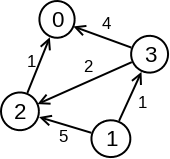
\includegraphics[scale=0.3]{slike/tezinski_graf.png}
\caption{Пример тежинског графа}
\label{fig:graf}
\end{figure}

\section{Дајкстрин алгоритам}

\subsection{Основна идеја}

Дајкстрин алгоритам одређује најкраћи пут од једног, унапред изабраног почетног чвора до свих осталих чворова у тежинском графу без грана негативне тежине.

\begin{definicija}
Нека је $d(v, u)$ дужина најкраћег пута од почетног чвора $v$ до чвора $u$. \emph{Релаксација} гране $(u, z)$ представља проверу да ли важи $$d(v, u) + w(u, z) < d(v, z),$$ и уколико важи, ажурирање тренутне процене $d(v, z)$ на мању вредност $d(v, u) + w(u, z)$.
\end{definicija}

Алгоритам гради решење постепено. На почетку је растојање до почетног чвора једнако $0$, а до свих осталих чворова једнако $+\infty$. У сваком следећем кораку бира се необрађени чвор са тренутно најмањом проценом растојања -- за тај чвор се показује да му је та процена уједно и коначна, најкраћа могућа вредност. Након тога се тај чвор проглашава обрађеним, а сви његови суседи се релаксирају. Поступак се понавља док се не обраде сви чворови.

\begin{teorema}
Ако граф $G$ нема грана негативне тежине, Дајкстрин алгоритам исправно одређује најкраћи пут од почетног чвора $v$ до сваког другог чвора у $G$.
\end{teorema}

\begin{napomena}
Уколико граф садржи гране негативне тежине, Дајкстрин алгоритам може дати погрешан резултат. У том случају се уместо њега користи, на пример, Белман--Фордов алгоритам.
\end{napomena}

\subsection{Псеудокод}

Извршавање алгоритма може се описати следећим корацима:

\begin{enumerate}
\item Растојање до почетног чвора поставити на $0$, а до свих осталих чворова на $+\infty$.
\item Све чворове сместити у ред са приоритетом, уређен према тренутној процени растојања.
\item Док год ред није празан, извући чвор $u$ са најмањом тренутном проценом растојања и прогласити га обрађеним.
\item За сваког суседа $z$ чвора $u$ извршити релаксацију гране $(u, z)$.
\item Вратити се на претходни корак све док се не обраде сви чворови.
\end{enumerate}

\subsection{Сложеност алгоритма}

Уколико се за имплементацију користи листа суседства и ред са приоритетом (хип), временска сложеност алгоритма износи $$O\big((n+m)\log n\big),$$ где је $n$ број чворова, а $m$ број грана графа. Захваљујући оваквој сложености, Дајкстрин алгоритам је применљив и на графове са великим бројем чворова и грана.

\section*{Закључак}

Дајкстрин алгоритам представља ефикасно решење проблема налажења најкраћих путева од једног чвора до свих осталих чворова у тежинском графу без грана негативне тежине. Захваљујући коришћењу реда са приоритетом, алгоритам постиже сложеност $O((n+m)\log n)$, због чега представља једну од основних техника које се изучавају у оквиру алгоритама на графовима.

\end{document}
